\documentclass{article}
\usepackage{ae,aecompl}
\usepackage{todonotes}
\usepackage{chngcntr}
\usepackage{tikz-cd}
\usepackage{graphicx}
\graphicspath{ {./images/}}
\usepackage[all,cmtip]{xy}
\usepackage{amsmath, amscd}
\usepackage{amsthm}
\usepackage{amssymb}
\usepackage{amsfonts}
\usepackage{bm}
\usepackage{qsymbols}
\usepackage{latexsym}
\usepackage{mathrsfs}
\usepackage{mathtools}
\usepackage{cite}
\usepackage{color}
\usepackage{url}
\usepackage{enumerate}
\usepackage{verbatim}
\usepackage[draft=false, colorlinks=true]{hyperref}
\usepackage{pdfpages}
\usepackage[margin=1.2in]{geometry}
\usepackage{IEEEtrantools}

\usepackage{fancyhdr}


\usepackage[nameinlink]{cleveref}


\DeclareMathOperator*{\ac}{accept}
\DeclareMathOperator*{\amax}{argmax}
\DeclareMathOperator*{\amin}{argmin}
\DeclareMathOperator*{\Aut}{Aut}
\newcommand {\al}{{\alpha}}
\newcommand {\abs}[1]{{\left\lvert#1\right\rvert}}
\newcommand {\A}{{\mathcal{A}}}
\newcommand {\AM}{{\mathrm{AM}}}
\newcommand {\AMp}{{\AM_{p}^{X}\!(\Ri_\w)}}
\newcommand {\B}{{\mathcal{B}}}
\DeclareMathOperator*{\Be}{Bern}
\newcommand {\Br}{{\dot{B}}}
\newcommand {\Ba}{{\mathfrak{B}}}
\newcommand {\C}{{\mathbb C}}
\newcommand {\ce}{\mathrm{c}}
\newcommand {\Ce}{\mathrm{C}}
\newcommand {\Cc}{\mathrm{C_{c}}}
\newcommand {\Ccinf}{\mathrm{C_{c}^{\infty}}}
\DeclareMathOperator{\cov}{Cov}
\DeclareMathOperator{\DEV}{DEV}
\newcommand {\Di}{{\mathbb D}}
\newcommand {\dom}{\mathrm{dom}}
\newcommand{\dist}{\stackrel{\mathrm{dist}}{=}}
\newcommand {\ud}{\mathrm{d}}
\newcommand {\ue}{\mathrm{e}}
\newcommand {\eps}{\varepsilon}
\newcommand {\veps}{\varepsilon}
\newcommand {\vrho}{{\varrho}}
\newcommand {\E}{{\mathbb{E}}}
\newcommand {\Ec}{{\mathcal{E}}}
\newcommand {\Ell}{L}
\newcommand {\Ellp}{{L_{p}[0,1]}}
\newcommand {\Ellpprime}{{L_{p'}([0,1])}}
\newcommand {\Ellq}{{L_{q}([0,1])}}
\newcommand {\Ellqprime}{{L_{q'}([0,1])}}
\newcommand {\Ellr}{L^{r}}
\newcommand {\Ellone}{{L_{1}([0,1])}}
\newcommand{\Elltwo}{{L_{2}([0,1])}}
\newcommand{\Ellinfty}{L^{\infty}}
\newcommand{\Ellinftyc}{L_{\mathrm{c}}^{\infty}}
\newcommand{\exb}[1]{\exp\left\{#1\right\}}
\DeclareMathOperator*{\Ext}{Ext}
\newcommand{\F}{{\mathcal{F}}}
\newcommand{\Fe}{{\mathbb{F}}}
\newcommand{\G}{{\mathcal{G}}}
\newcommand{\HF}{\mathcal{H}_{\text{FIO}}^{1}(\Rd)}
\newcommand{\Hr}{H}
\newcommand{\HT}{\mathcal{H}}
\newcommand{\ui}{\mathrm{i}}
\newcommand{\I}{{I}}
\newcommand{\J}{{\mathcal{J}}}
\newcommand{\id}{{\mathrm{id}}}
\newcommand{\iid}{\stackrel{\mathclap{\normalfont\mbox{iid}}}{\sim}}
\newcommand{\im}{{\text{im }}}
\newcommand{\ind}{{\perp\!\!\!\perp}}
\DeclareMathOperator*{\Int}{int}
\newcommand{\intx}{{\overline{\int_{X}}}}
\newcommand{\inte}{{\overline{\int_{\E}}}}
\newcommand{\la}{\lambda}
\newcommand{\rb}{\rangle}
\newcommand{\lb}{{\langle}}
\newcommand{\La}{\Lambda}
\newcommand{\calL}{{\mathcal{L}}}
\newcommand{\lp}{{\mathcal{L}}^{p}}
\newcommand{\lpo}{{\overline{\mathcal{L}}^{p}\!}}
\newcommand{\Lpo}{{\overline{\Ell}^{p}\!}}
\newcommand{\M}{{\mathbf{M}}}
\newcommand{\Ma}{{\mathcal{M}}}
\newcommand{\N}{{{\mathbb N}}}
\newcommand{\Na}{{{\mathcal{N}}}}
\newcommand{\norm}[1]{\left\|#1\right\|}
\newcommand{\normm}[1]{{\left\vert\kern-0.25ex\left\vert\kern-0.25ex\left\vert #1 
    \right\vert\kern-0.25ex\right\vert\kern-0.25ex\right\vert}}
\newcommand{\Om}{{{\Omega}}}
\newcommand{\one}{{{\bf 1}}}
\newcommand{\pic}{\text{Pic }}
\newcommand{\ph}{{\varphi}}
\newcommand{\Pa}{{\mathbb{P}}}
\newcommand{\Po}{{\mathcal{P}}}
\newcommand{\Q}{{\mathbb{Q}}}
\newcommand{\R}{{\mathbb R}}
\newcommand{\Rd}{{\mathbb{R}^{d}}}
\DeclareMathOperator{\rej}{reject }
\newcommand{\Rn}{{\mathbb{R}^{n}}}
\newcommand{\cR}{{\mathcal{R}}}
\newcommand{\Rad}{{\mathrm{Rad}}}
\newcommand{\ran}{{\mathrm{ran}}}
\newcommand{\Ri}{{\mathrm{R}}}
\newcommand{\supp}{{\mathrm{supp}}}
\newcommand{\Se}{\mathrm{S}}
\newcommand{\Sp}{S^{*}(\Rn)}
\newcommand{\St}{{\mathrm{St}}}
\newcommand{\Sw}{\mathcal{S}}
\newcommand{\T}{{\mathcal{T}}}
\newcommand{\ta}{{\theta}}
\newcommand{\Ta}{{\Theta}}
\newcommand{\topp}{\stackrel{p}{\to}}
\newcommand{\todd}{\stackrel{d}{\to}}
\newcommand{\toL}[1]{\stackrel{L^{#1}}{\to}} 
\newcommand{\toas}{\stackrel{a.s.}{\to}}
\DeclareMathOperator{\V}{Var}
\newcommand {\w}{{\omega}}
\newcommand {\W}{{\mathrm{W}}}
\newcommand {\Wnp}{\text{$\mathrm{W}$\textsuperscript{$n,\!p$}}}
\newcommand {\Wnpeq}{\text{$\mathrm{W}$\textsuperscript{$n\!,\!p$}}}
\newcommand {\Wonep}{\text{$\mathrm{W}$\textsuperscript{$1,\!p$}}}
\newcommand {\Wonepeq}{\text{$\mathrm{W}$\textsuperscript{$1\!,\!p$}}}
\newcommand {\X}{{\mathcal{X}}}
\newcommand {\Z}{{{\mathbb Z}}}
\newcommand {\Za}{{\mathcal{Z}}}
\newcommand {\Zd}{{\Z[\sqrt{d}]}}
\newcommand {\vanish}[1]{\relax}

\newcommand {\wh}{\widehat}
\newcommand {\wt}{\widetilde}
\newcommand {\red}{\color{red}}

% Distributions
\newcommand{\normal}{\mathsf{N}}
\newcommand{\poi}{\mathsf{Poisson}}
\newcommand{\bern}{\mathsf{Bernoulli}}
\newcommand{\bin}{\mathsf{Binomal}}
\newcommand{\multi}{\mathsf{Multinomial}}
\newcommand{\Exp}{\mathsf{Exp}}



% put your command and environment definitions here




% some theorem environments
% remove "[theorem]" if you do not want them to use the same number sequence


  \newtheorem{thrm}{Theorem}
  \newtheorem{lemma}{Lemma}
  \newtheorem{prop}{Proposition}
  \newtheorem{cor}{Corollary}

  \newtheorem{conj}{Conjecture}
  \renewcommand{\theconj}{\Alph{conj}}  % numbered A, B, C etc

  \theoremstyle{definition}
  \newtheorem{defn}{Definition}
  \newtheorem{ex}{Example}
  \newtheorem{exs}{Examples}
  \newtheorem{question}{Question}
  \newtheorem{remark}{Remark}
  \newtheorem{notn}{Notation}
  \newtheorem{exer}{Exercise}




\title{STATS305A - Lecture 9}
\author{John Duchi\\ Scribed by Michael Howes}
\date{10/19/21}

\pagestyle{fancy}
\fancyhf{}
\rhead{STATS305A - Lecture 9}
\lhead{10/19/21}
\rfoot{Page \thepage}

\begin{document}
\maketitle
\tableofcontents
\section{Recap}
Recall our testing framework: we compute a test statistic $t_{obs}$, under the null $H_0$ $t_{obs}$ follows some distribution $T$, reject if the $p$-value is less than some threshold, i.e. $\Pa_{H_0}(T \ge t_{obs}) \le \al$.
\section{Chosing alternative hypotheses}
See ``Strong Inference'' by John Platt 60s/70s in Science. 

When designing a test, it is very important to consider alternatives to the null hypothesis and design a tst to \emph{best} distinguish your null $H_0$ from possible alternatives.

\subsection{Neymann-Pearson}
Suppose that we have point null and alternative hypotheses and so 
\begin{align*}
    H_0&:X \sim \Pa_0,\\
    H_1&:X \sim \Pa_1.
\end{align*}
\underline{Question:} For a given level $\al \in (0,1)$ (ie $\Pa_0(\text{reject }H_0) \le \al$), what is the best test to distinguish $\Pa_0$ and $\Pa_1$ i.e. which test maximizes the power
\[\beta := \Pa_1(\text{reject} H_0). \]
\underline{Answer:} The Neymann-Pearson lemma (NPL). Say $P_0, P_1$ have densities $p_0(x)$ and $p_1(x)$, define
\[L(x) = \log\left(\frac{p_1(x)}{p_0(x)}\right). \]
The optimal test is given by choosing a threshold $t_\al$ such that we 
\begin{itemize}
    \item Reject $H_0$ (accept $H_1$) if $L(X) > t_\al$.
    \item Reject $H_1$ (accpet $H_0$ (not reject $H_0$)) if $L(X) < t_\al$.
    \item Randomly reject/accept $H_0$ with equal probability if $L(X) = t_\al$.
\end{itemize}
Where we choose $t_\al$ to be the smallest $t$ such that 
\[\Pa_0(L(X) >t) \le \al. \]
For the proof, see Wikipedia. 

How do we use this in practice? We pick a null $H_0$, we think about possible alternatives, choose a test which distinguishes them and we can use NP to decide on the choice of test.
\begin{ex}
    Suppose we want to test a treatment/intervention in some setting. For example we might want to
    \begin{enumerate}
        \item Create a drug that treats obesity.
        \item Set a harder final exam.
    \end{enumerate}
    In (a) we are interested in a change in weight. We wish to see if the mean weight of the treated population decreases. In (b) we want to increase the spread to better assign grades. We wish to see if the variance increases. 

    Suppose that the null in both cases is
    \[X_i \iid \Na(0,1). \]
    The alternative in (a) is the mean decreases to $\mu <0$ so $X_i \iid \Na(\mu,1)$. The alternative in (b) is the variance of $X_i$ increases to $\sigma^2 >1$ so $X_i \iid \Na(0,\sigma^2)$.

    Let $x=(x_i)_{i=1}^n$, then in (a)
    \begin{align*}
        L(x)& = -\frac{1}{2}\sum_{i=1}^n(x_i-\mu)^2 +\frac{1}{2}\sum_{i=1}^n x_i^2\\
            & = -\sum_{i=1}^n x_i \mu + \frac{n}{2}\mu^2\\
            &= -\frac{n}{2}\mu^2 + n \mu \bar{x}_n.
    \end{align*}
    By NPL the opitimal test is of the form reject $H_0$ if $L(x) > t_\al$ where $t_\al$ satisfies
    \begin{align*}
        \Pa_0(L(X) \ge t_\al) &=\al.
    \end{align*}
    Note that since $\mu < 0$,
    \begin{align*}
        \Pa_0(L(X) \ge t_\al) &=\Pa_0\left(-\frac{n}{2}\mu^2+n\bar{X}_n \mu \ge t_\al \right)\\
        &=\Pa_0\left(-n\bar{X}_n \mu \le -\frac{n}{2}\mu^2-t_\al \right)\\
        &=\Pa_0\left(\sqrt{n}\bar{X}_n \le \frac{\sqrt{n}}{2}-\frac{t_\al}{\mu\sqrt{n}}\right).
    \end{align*}
    We know that $\sqrt{n}\bar{X}_n \sim \Na(0,1)$ under $H_0$. Thus we set $\frac{\sqrt{n}}{2}-\frac{t_\al}{\mu\sqrt{n}} = -z_{1-\al}$ where $z_{1-\al}$ is the $1-\al$ quantile of $\Na(0,1)$. Thus NPL says we should reject when $\sqrt{n} \bar{x}_n \le - z_{1-\al}$. Thus we reject when the sample mean is negative which makes sense.

    In (b) note that
    \begin{align*}
        L(x)&=-\frac{1}{2\sigma^2}\sum_{i=1}^n x_i^2 + \frac{1}{2}\sum_{i=1}^n x_i^2 + \frac{1}{2}\log(\sigma^2)\\
        &=\frac{1}{2}\left(1-\frac{1}{\sigma^2}\right)\sum_{i=1}^n x_i^2 + \log(\sigma).
    \end{align*}
    We know that $\sigma^2 > 1$ and so $1-\frac{1}{\sigma^2} > 0$. Thus the NP test rejects when $\sum_{i=1}^n x_i^2$ is greater than some threshold. Under the null, $\sum_{i=1}^n X_i^2$ follows a $\chi^2_{(n)}$ distribution. Thus the optimal level $\al$ test rejects when 
    \[\sum_{i=1}^n x_i^2 \ge \chi^2_{n,\al}. \]
\end{ex}
    What if our $H_0$ is \emph{not} a point null e.g. $H_0 : X_i \iid N(0,\sigma^2)$ with $\sigma^2$ unknown. Neymann Pearson does not apply. The ``solution'' is to use a plug-in estimate. That is estimate the unkown parameters, plug them in and then use Neymann-Pearson and other similiar methods. This is the idea behind the $t$-test when we compute
    \[t_n := \frac{\sqrt{n}\bar{X}_n}{S_n}, \]
    where $S_n^2 =\frac{1}{n-1}\sum_{i=1}^n (X_i-\bar{x}_n)^2$.
\subsection{ANOVA}
Let's us again consider contrasts in the ANOVA model. We have $Y_{i,j} = \mu + \al_i + \eps_{i,j}$ where $i=1,\ldots, k$ and $j=1,\ldots, n_i$. We are interested in the nulls $H_{0,i} : \al_i =0$ where $i=1,\ldots, k$. We know the estimable constrasts are $\la^T \bar{Y}$ where $\la \in R^k$ and $\la^T \one = 0$ but $\la \neq 0$ where 
\[\bar{Y} = \begin{bmatrix}
    \bar{Y}_{1,\bullet} \\ \vdots \\ \bar{Y}_{k,\bullet}
\end{bmatrix} \in \R^k. \]
Under $H_0 : \al_i = 0$ for all $i$ and $\eps_{i,j} \iid \Na(0,\sigma^2)$ we have $\la^T \bar{Y} \sim \Na(0, \sum_{i=1}^n \la_i^2/\sqrt{n_i})$. We can ask what is the most powerful test of $\al \neq 0$? It turns out it dos not exist since $H_1 : \al \neq 0$ is not  point hypothesis.
\begin{defn}
    The \emph{non-central $\chi^2$ distribution} is written $\chi_{(n),NC}^2(\norm{u}_2^2)$ is the distribution of $\norm{Z}_2^2$ where $Z \sim \Na(\mu,I_n)$. Note that this distribution only depends on $n$ and $\norm{u}_2^2$ since 
    \begin{align*}
        \norm{z}_2^2&= \norm{u+z-u}_2^2\\
        &= \norm{z-u}_2^2 +2u^T(z-u) +\norm{u}_2^2\\
        &= \norm{z-u}_2^2 +2\norm{u}_2\left(\frac{u}{\norm{u}_2}\right)^T(z-u) +\norm{u}_2^2.
    \end{align*}
\end{defn}
If $\al \neq 0$, then 
\begin{align*}
    \frac{(\la^T \bar{Y})^2}{\sum_{i=1}^n \frac{\la_i^2}{n_i}}&=\left(\sum_{i=1}^n \frac{\la_i \al_i}{\sqrt{\sum_{i=1}^n \la_i^2/n_i}}-\frac{\la^T(\bar{Y}-\al)^2}{\sqrt{\sum_{i=1}^n \la_i^2/n_i}}\right)^2 \\
    &\stackrel{dist}{=} \left(\frac{\la^T\al}{\sqrt{\sum_{i=1}^n \la_i^2/n_i}}+N(0,1)^2\right)\\
    &\sim \chi^2_{(1), NC}\left(\left(\frac{\la^T\al}{\sqrt{\sum_{i=1}^n \la_i^2/n_i}}\right)^2\right).
\end{align*}
Thus the distribution of our statistic under $H_1$ depends on $\al$ and thus the test which maximizes power also depends on $\al$. (One way ``around'' this issue: split the data use half to estimate $\wh{\al}$ and use the other half to test $H_0 : \al=0$ against $H_1 : \al = \wh{\al}$. This assumes that we can split the data into two independent halves).
\section{Multiple testing}
Can we correctly get some of the ``discoveries'' in a sample without making too many mistakes? 

\subsection{Setting}
We have many nulls $H_{0,j}$, $j=1,\ldots k$, correctly rejecting a null equals making a discovery. A typical example is $(H_{0,j}:Y=X\beta+\eps, \beta_j = 0$). We want to control \emph{false discoveries} where we reject $H_{0,j}$ even though $H_{0,j}$ is true.

\subsection{Family wise error rate (FWER)}
When we look at the FWER no mistakes are allowed. In this setting we can use Bonferroni correction and reject $H_{0,j}$ with at the level $\al/k$. In this case
\[\Pa(\text{one or more false rejections}) \le \sum_{j=1}^k \Pa(H_{0,j} \text{ falsely rejected}) \le \frac{k\al}{k} = \al. \]
This is quite strict. Maybe we should be willing to make some false discoveries if it allows us to make more true discoveries.

\subsection{False discovery proportion (FDP)}
Define
\[FDP:= \frac{\#\{\text{false rejections}\}}{\#\{\text{rejections}\} \lor 1}, \]
where $a\lor b = \max\{a,b\}$. Controlling FDP means we are allowing overselves to make some mistakes if it means we make more true discoveries. Define the FDR (false discovery rate) to be
\[FDR = \E[FDP].\]
We will try to control FDR rather than FWER. 
\begin{aside}
    What is the distribution of $p$-value under the null $H_0$? It should be uniform on $[0,1]$ or ``larger''. This is because if $F$ is the CDF of a random variable $X$ then 
    \begin{align*}
        \Pa(F(X) \le u) &= \Pa(X \le F^{-1}(u))\\
        &=F(F^{-1}(u))\\
        &=\begin{cases}
            u & \text{if } X \text{ has a density},\\
            \ge u & \text{else}.
        \end{cases}
    \end{align*}
    where $F^{-1}(u) = \inf\{t: F(t) \ge u \}$. See picture for a CDF with a jump at a value $x_0$.

    \begin{center}
        
\includegraphics[width = \textwidth]{10_19_P01.jpg}
    \end{center}
    
    Now if we think about $p$-values. If $F$ is a CDF of the test-statistic $T$ under $H_0$ we reject for $T$ large. Thus $p = 1-F(t_{obs})$ where $t_{obs}$ is our observed test-statistic. Thus 
    \begin{align*}
        \Pa_0(p<u)&= \Pa_0(1-F(t_{obs})<u)\\
        &=\Pa_0(F(t_{obs})>1-u)\\
        &=1-\Pa_0(F(t_{obs})\le 1-u)\\
        &\le 1-(1-u)\\
        &=u.
    \end{align*}
    And we have equality if $F$ is continuous.
\end{aside}
Going back to our multiple testing setting. Suppose we collect a pile of $p$-values $p_1,\ldots, p_k$ and make a histogram. It would look like this

\begin{center}
    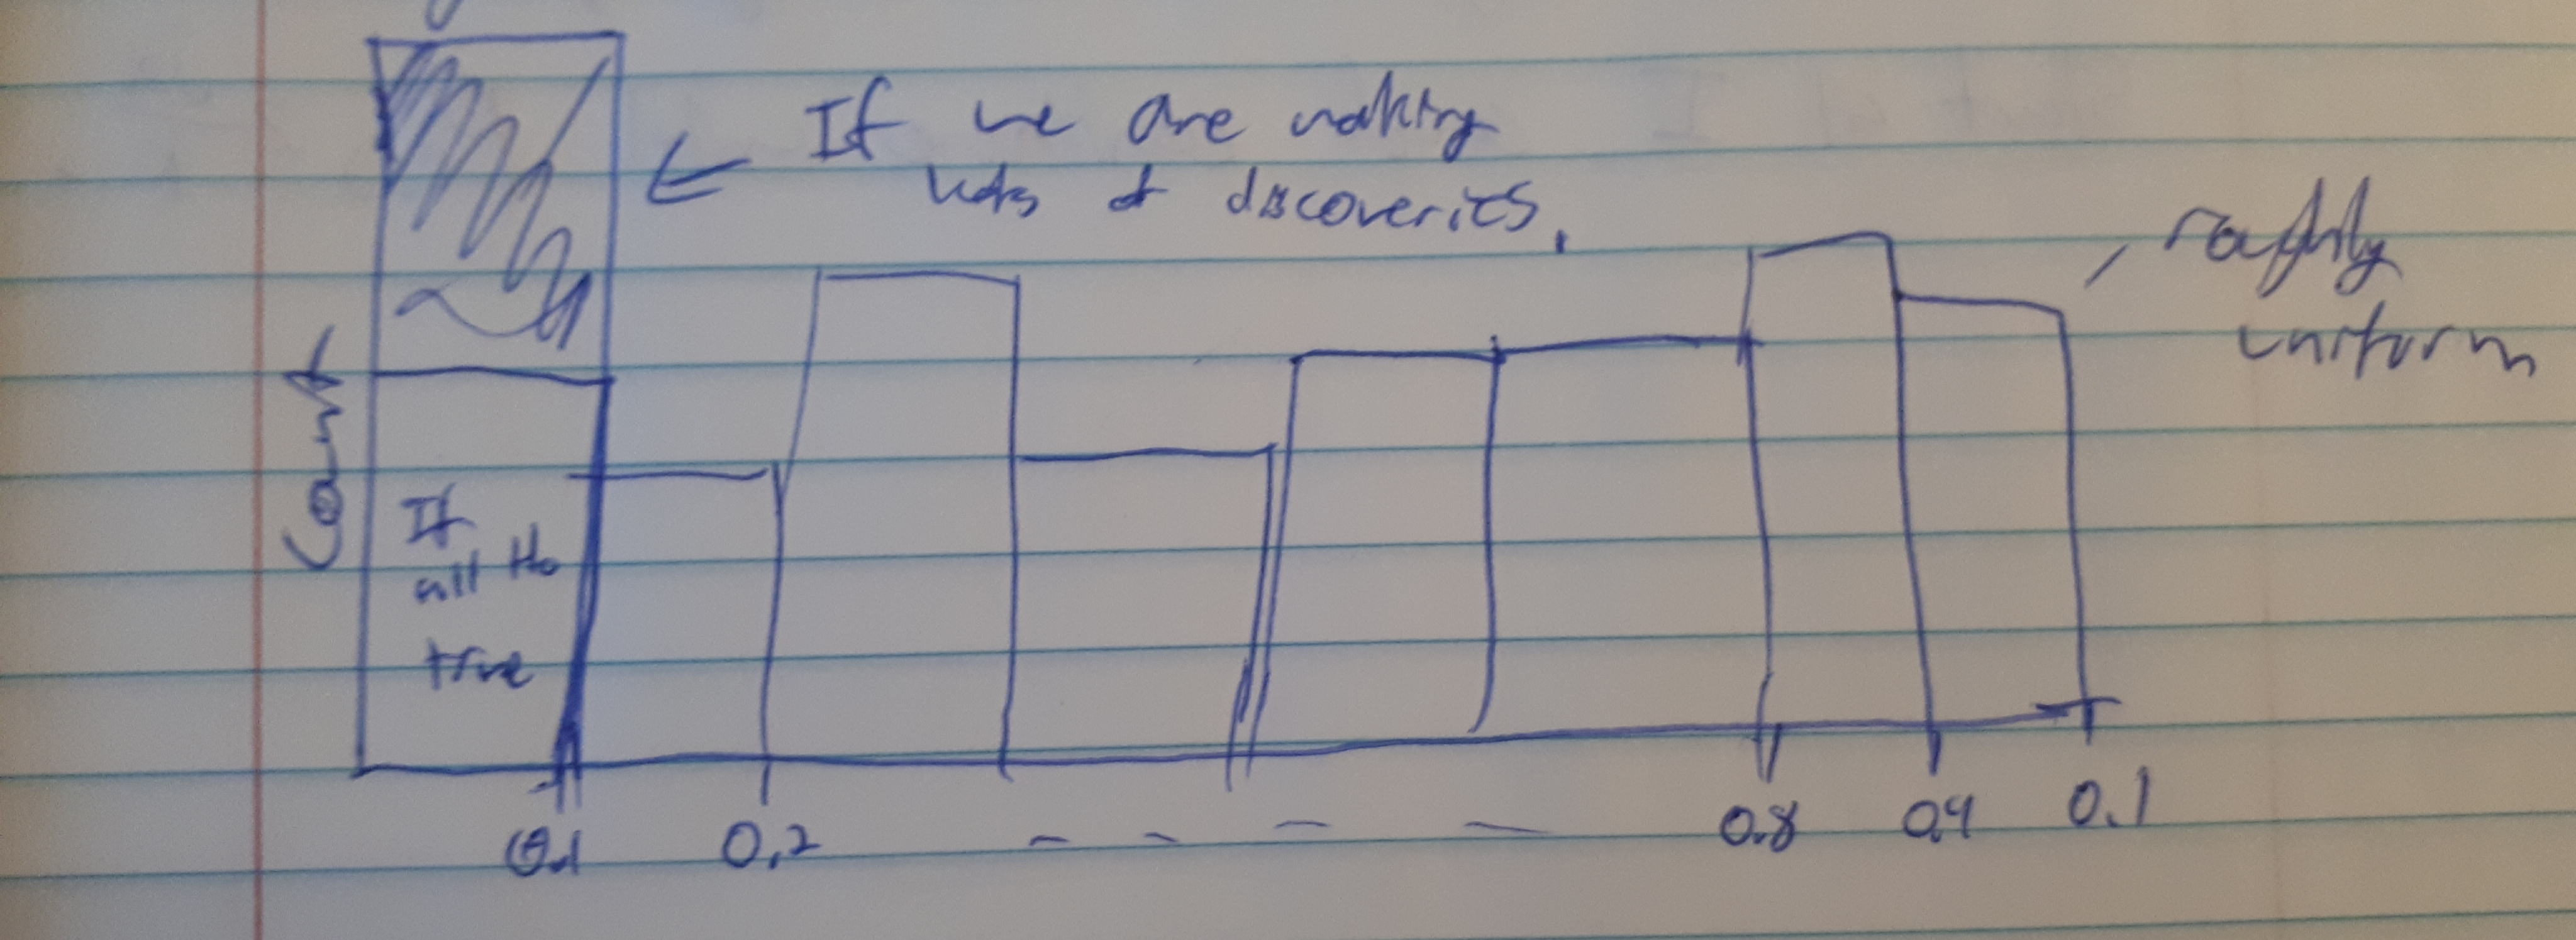
\includegraphics[width = \textwidth]{10_19_P02.jpg}
\end{center}

We would expect a roughly uniform distribution for most values of $p$ but for small values there should be a spike corresponding to all the nulls we should reject. If we sort the $p$-value and plot them we'll get something like this:

\begin{center}
    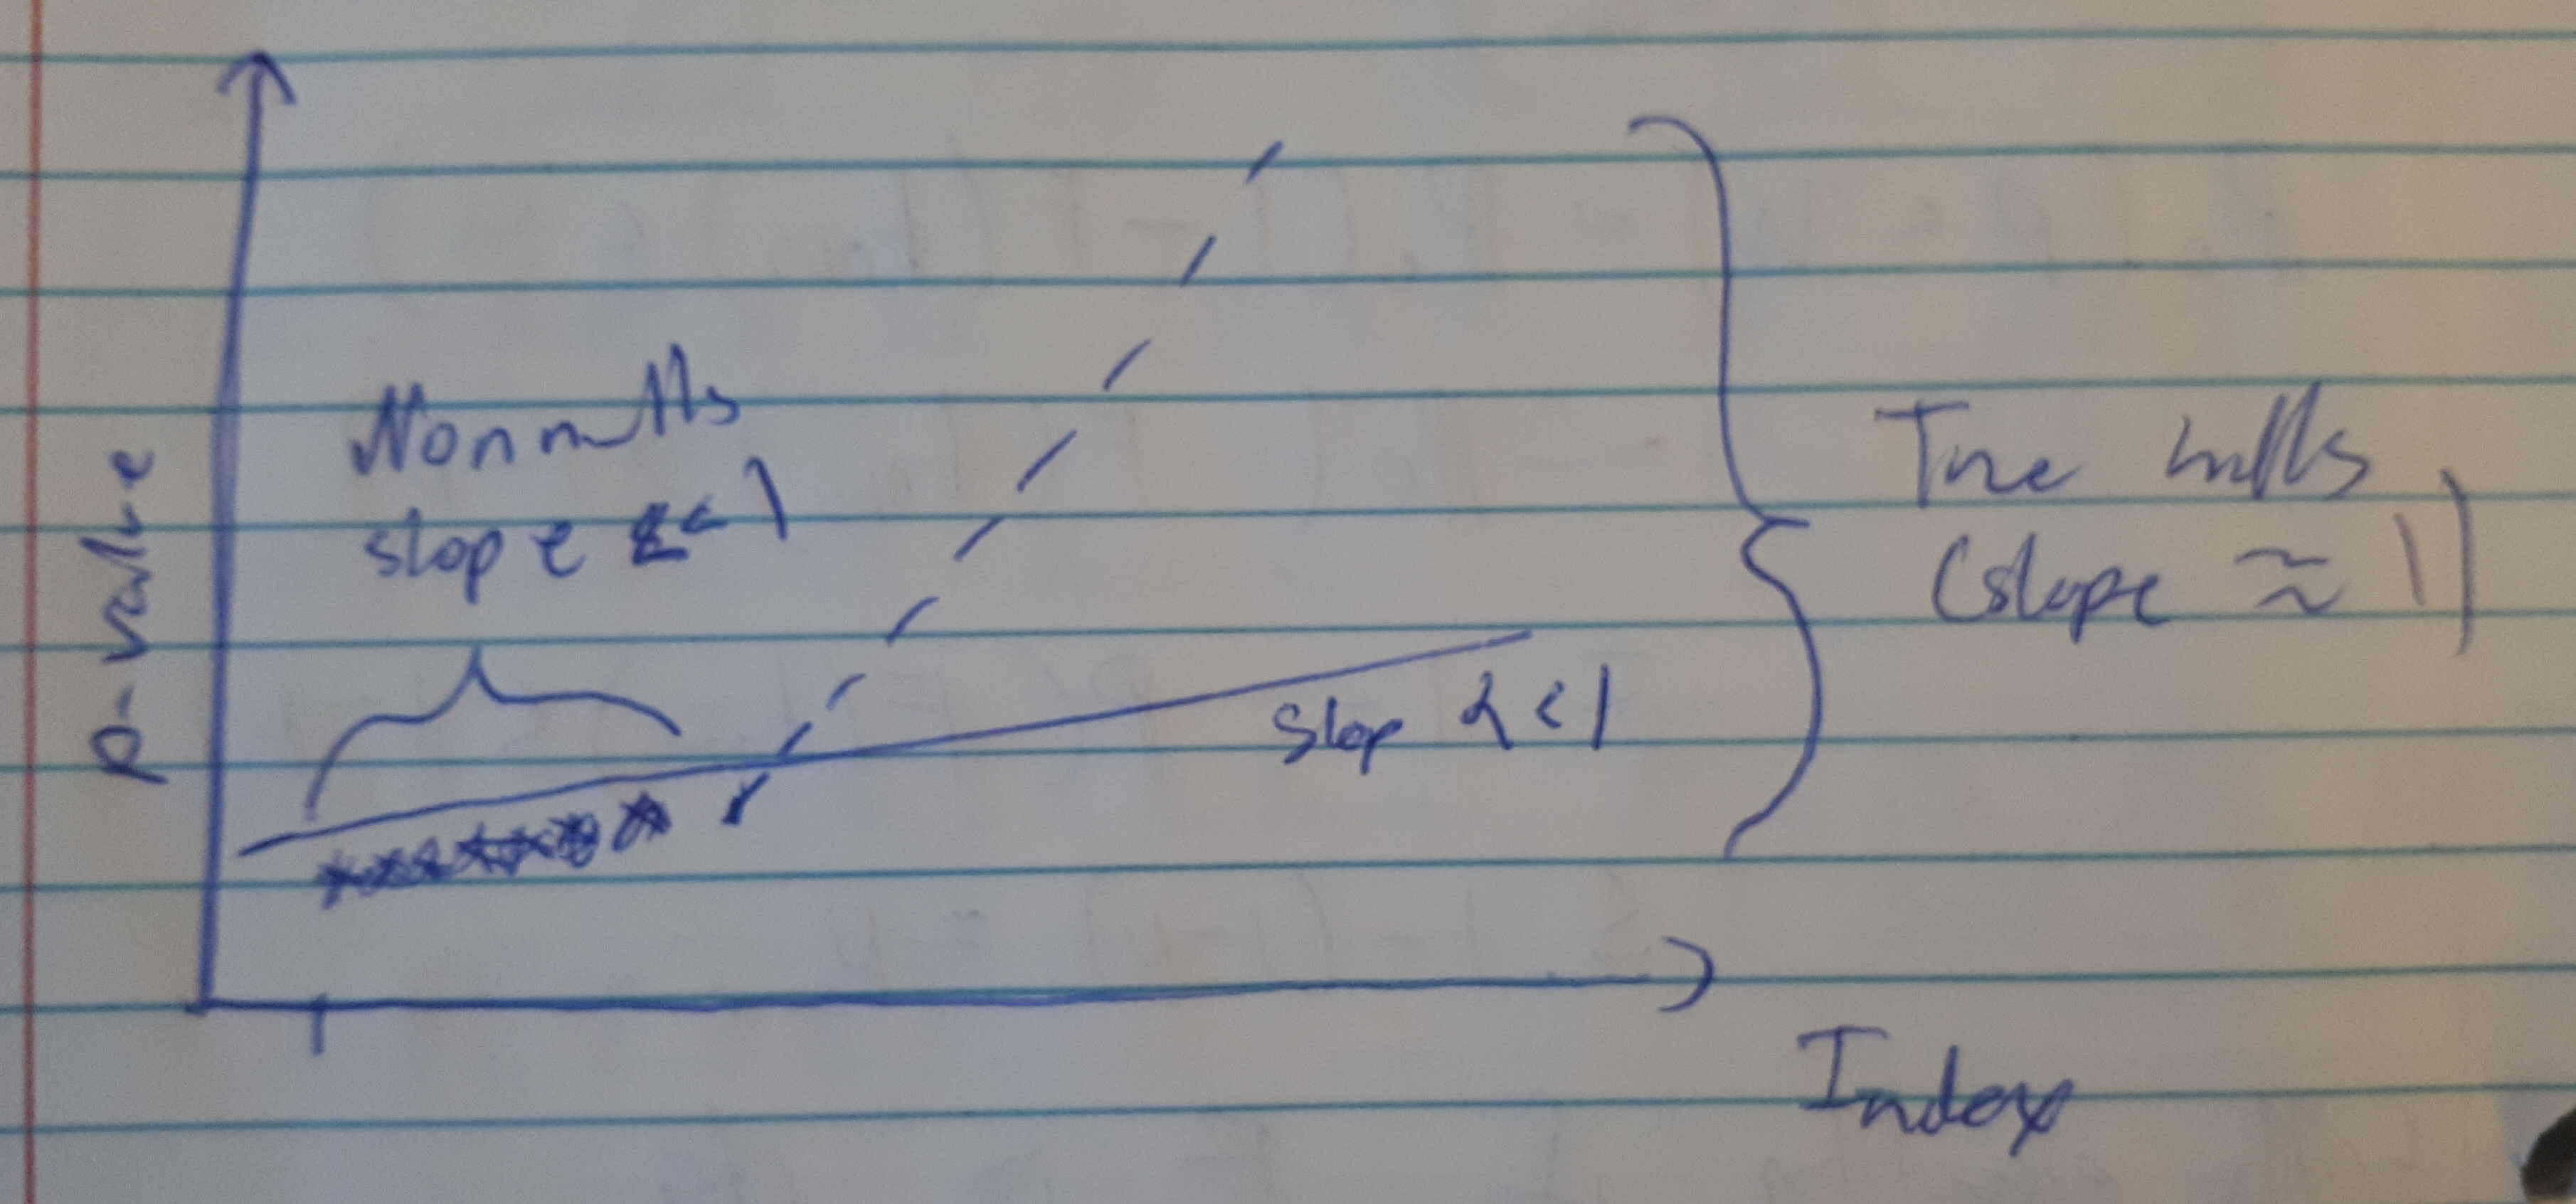
\includegraphics[width = \textwidth]{10_19_P03.jpg}
\end{center}

For the true nulls, the slope will be approximately 1 but the slope will be much flatter for the $p$-values corresponding to false nulls. We reject the nulls that fall below the slope $\al$ line. This is the \emph{Benjamini Hochberg procedure}. We start at $p_{(1)}$ and reject the nulls until $p_{(j)} \ge \frac{j\al}{k}$.
\end{document}